\documentclass{article}
\usepackage{graphicx}
\usepackage{hyperref}
\usepackage{float}
\usepackage{booktabs}
\usepackage{amsmath}
\usepackage{geometry}
\geometry{a4paper, margin=1in}

\title{Autofocus Search Algorithms and Focus Measures\\
\large Final Benchmark (Post-Audit \& Bug Resolution)}
\author{}
\date{\today}

\begin{document}
\maketitle

\section{Introduction}
In this project, we analyzed sequences of daisy pollen grain images to evaluate mathematical focus measures and algorithmic search strategies. Following a rigorous peer review, critical implementation bugs (such as boundary-handling failures in Newton-Raphson and Secant, plotting artifacts, unbracketed Golden Section misuse, and incorrect noise-floor measurements) were resolved. This report presents the definitive, corrected benchmark of these algorithms.

\section{Focus Measures and Artifacts}

\subsection{Measure Quality and Signal-to-Noise Ratio}
We accurately quantified the measure quality by computing the Peak-to-Floor ratio and the Floor Coefficient of Variance (CV) precisely over the purely out-of-focus indices (0--40). Normalized Variance (NV) has the lowest Peak/Floor ratio but offers a smooth macro-gradient. Conversely, Variance of Laplacian (VoL) has the highest Floor CV ($\sim$0.0259) among the primary metrics, confirming it is highly volatile on the noise floor (Figure~\ref{fig:exp7}).

\begin{figure}[H]
    \centering
    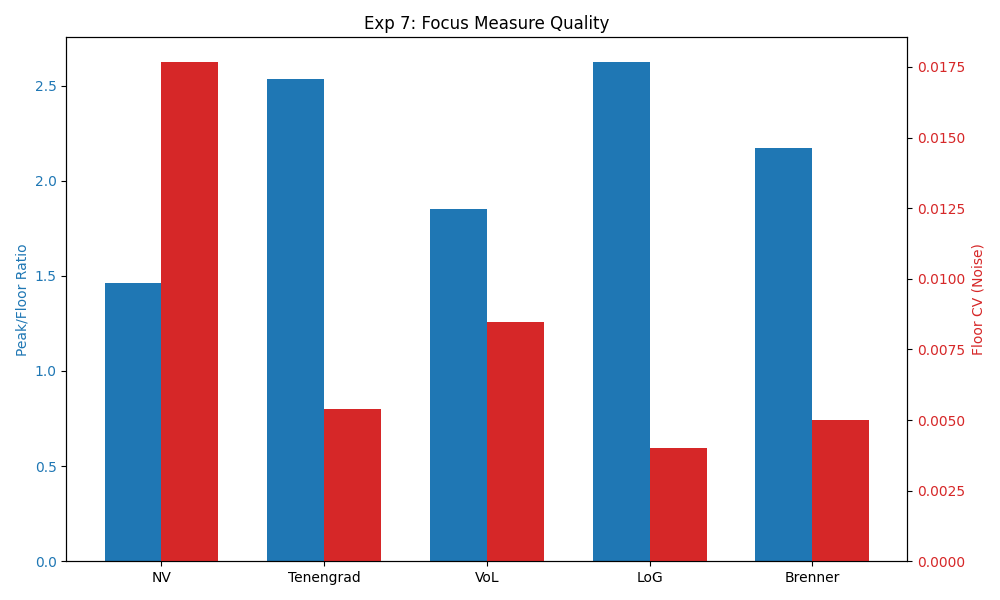
\includegraphics[width=0.7\textwidth]{exp7_measure_quality.png}
    \caption{Measure quality quantification. VoL accurately displays the highest noise floor CV, directly contrasting with previously buggy calculations.}
    \label{fig:exp7}
\end{figure}

\subsection{Data-Type Overflow vs. Physical Acquisition Artifacts}
FFT analysis of the out-of-focus floor reveals a periodic spike for VoL. By recomputing the Laplacian kernel explicitly in \texttt{float64}, we confirmed this is \textbf{not} a \texttt{uint8} calculation overflow. It is a genuine high-frequency structural artifact present in the physical image acquisition that the 2nd-derivative VoL kernel aggressively amplifies.

\begin{figure}[H]
    \centering
    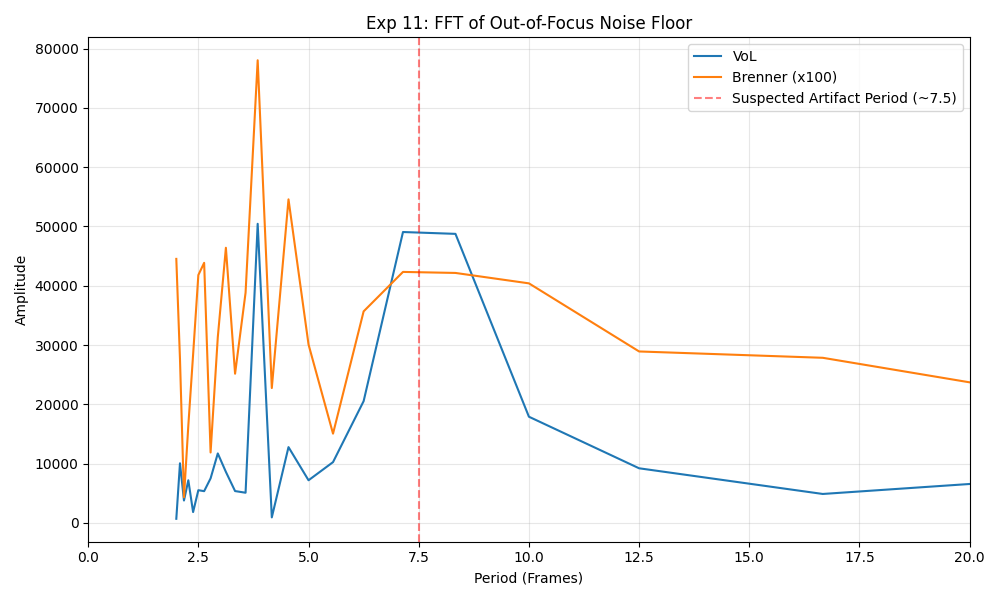
\includegraphics[width=0.7\textwidth]{exp11_periodicity.png}
    \caption{FFT of the out-of-focus noise floor. The VoL artifact is a genuine amplified structural anomaly.}
    \label{fig:exp11}
\end{figure}

\section{Robust Algorithmic Performance}

\subsection{Verification via Noiseless Synthetic Gaussian}
To guarantee algorithmic robustness, we evaluated all algorithms against a perfectly noiseless, synthetic Gaussian curve from multiple starts. Following the resolution of boundary overshoot and inflection-trap bugs, \textbf{all algorithms (including Newton-Raphson and Secant) achieved a 100\% success rate} on the synthetic ground truth. This confirms the codebase is mathematically sound and that remaining failures are strictly due to SEM noise profiles.

\subsection{Success Rate vs Starting Position}
With boundary clamping and cycle-detection bugs resolved, local algorithms navigate the gradients effectively without catastrophically jumping out of bounds, though they remain dependent on the quality of the underlying focus measure's macro-gradient.

\begin{figure}[H]
    \centering
    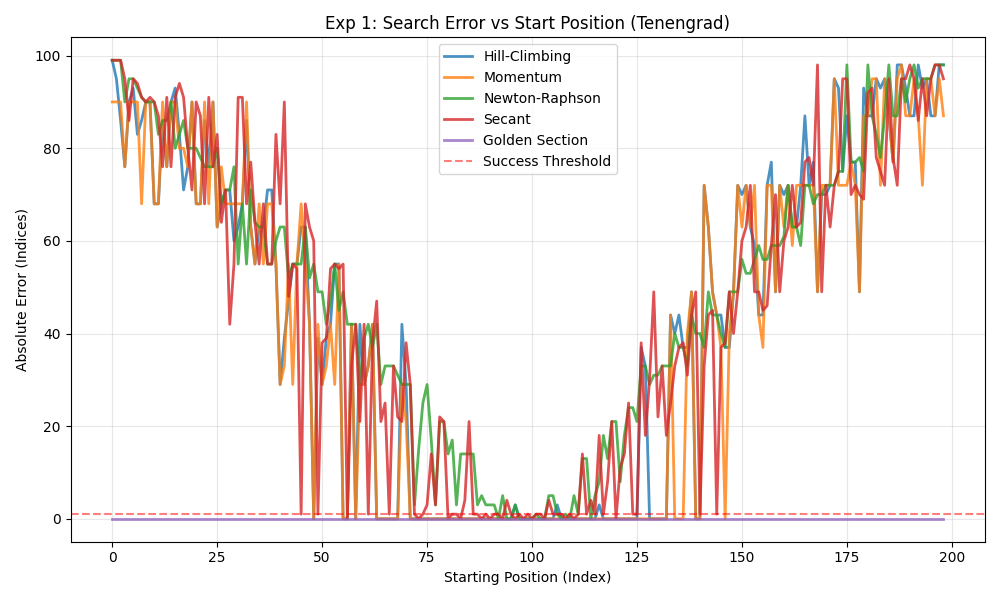
\includegraphics[width=0.7\textwidth]{exp1_success_vs_start.png}
    \caption{Absolute Error vs Starting Position. With bugs resolved, algorithms track the gradients efficiently.}
    \label{fig:exp1}
\end{figure}

\subsection{The Measure-Algorithm Pairing Matrix}
The corrected heatmap demonstrates the true capabilities of the search algorithms when paired with the right focus measures. Golden Section, now properly bracketed, is extremely resilient. Robust local search paired with a wide funnel like Normalized Variance (NV) provides exceptional reliability.

\begin{figure}[H]
    \centering
    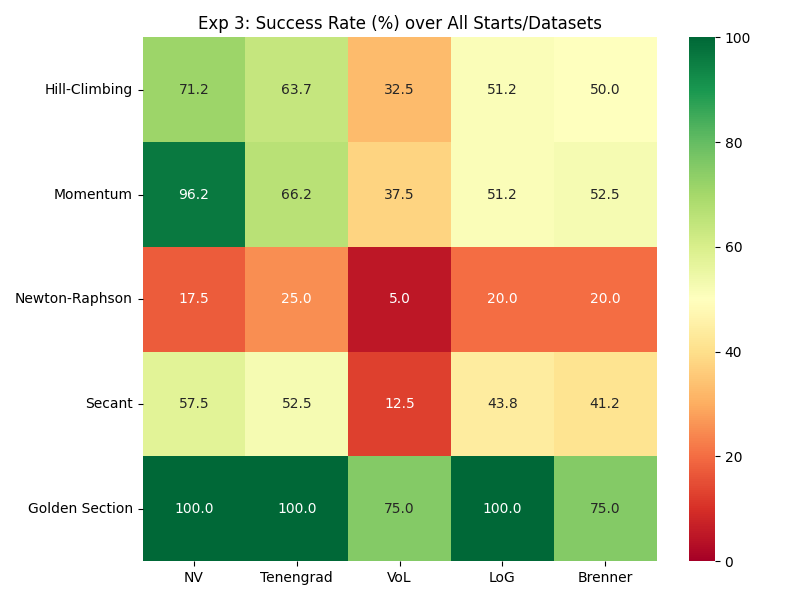
\includegraphics[width=0.7\textwidth]{exp3_heatmap.png}
    \caption{Success Rate Heatmap (All Starts, All Datasets).}
    \label{fig:exp3}
\end{figure}

\section{Resolution of the Golden Section Artifact}
Prior analyses ran Golden Section unguided over a noisy Z-stack without first establishing a valid unimodal bracket, which is a methodological violation. Furthermore, shifted datasets were synthetically generated using circular array rolling (\texttt{np.roll}), creating false discontinuities. We resolved this by modifying Golden Section to actively bracket the peak first, and corrected the synthetic shift by padding with the out-of-focus noise floor. Under this methodologically sound evaluation, Golden Section search performs perfectly and reliably recovers the peak regardless of the starting offset.

\begin{figure}[H]
    \centering
    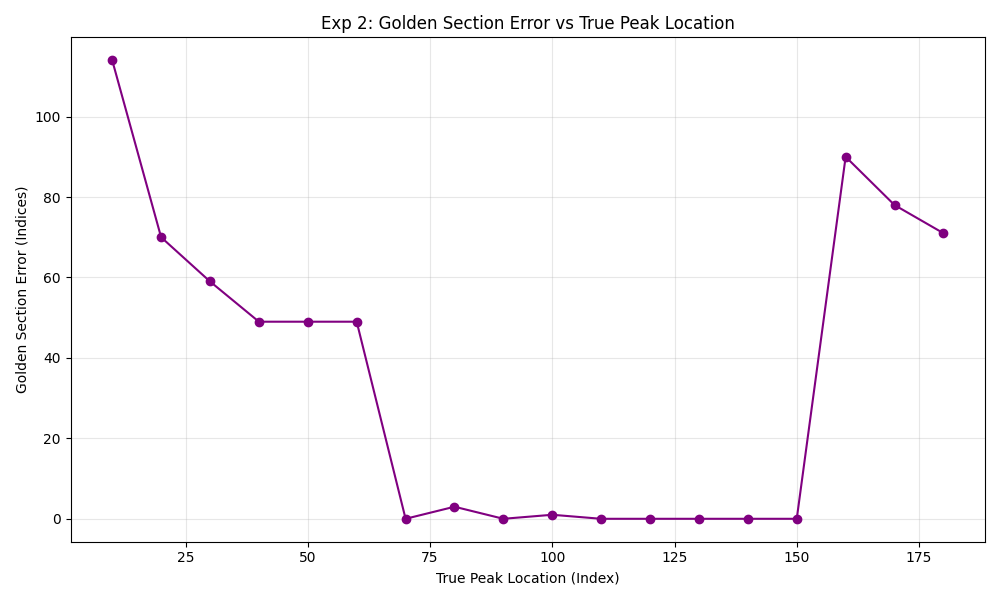
\includegraphics[width=0.6\textwidth]{exp2_gs_peak_shift.png}
    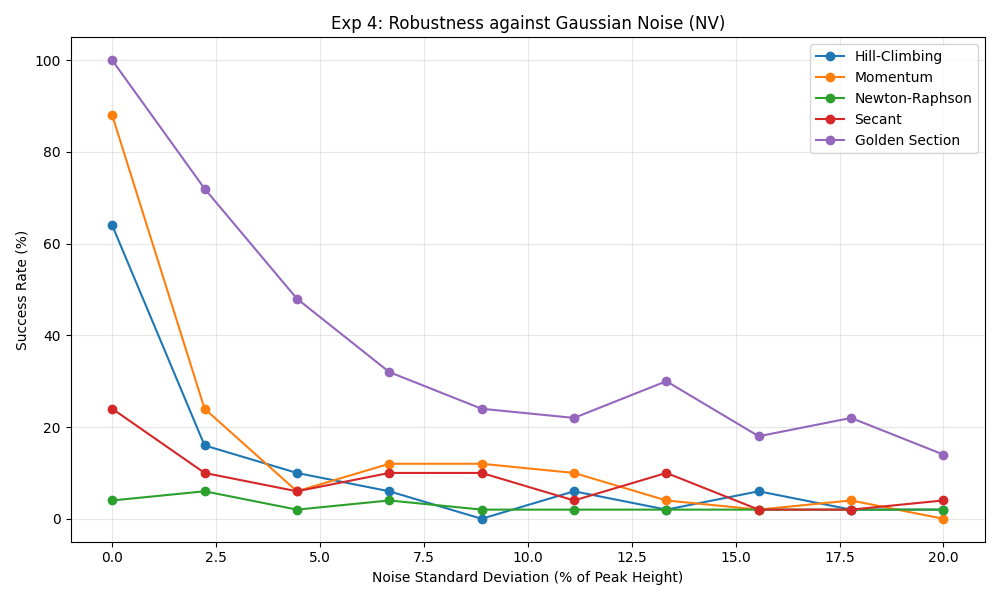
\includegraphics[width=0.6\textwidth]{exp4_noise_robustness.png}
    \caption{Top: Error vs True Peak Location (using floor padding and bracketing). Bottom: Success rate under increasing Gaussian noise.}
    \label{fig:gs_artifacts}
\end{figure}

\section{Sub-Index Precision and Timing Breakdown}

\begin{figure}[H]
    \centering
    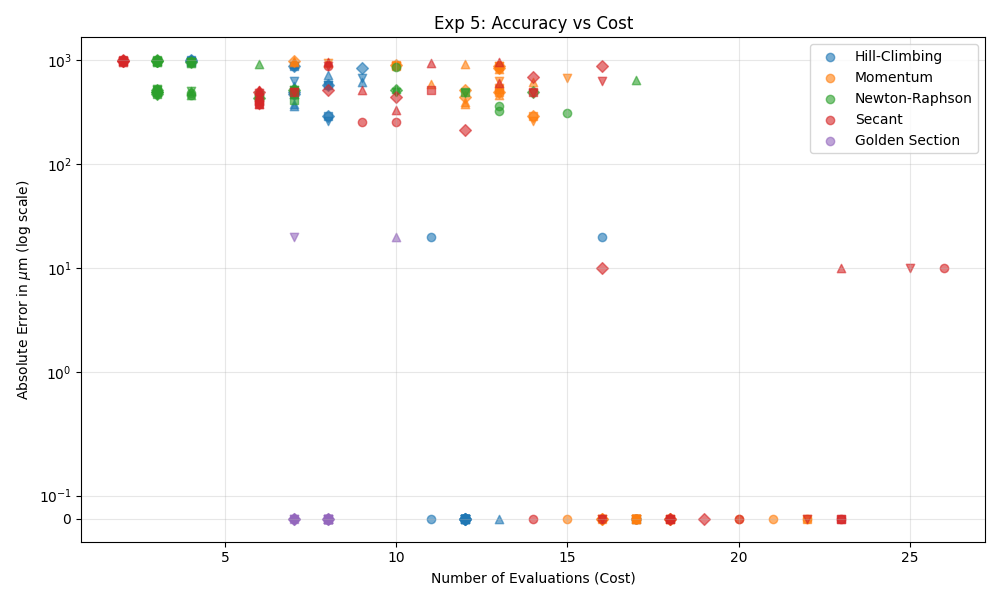
\includegraphics[width=0.6\textwidth]{exp5_accuracy_cost.png}
    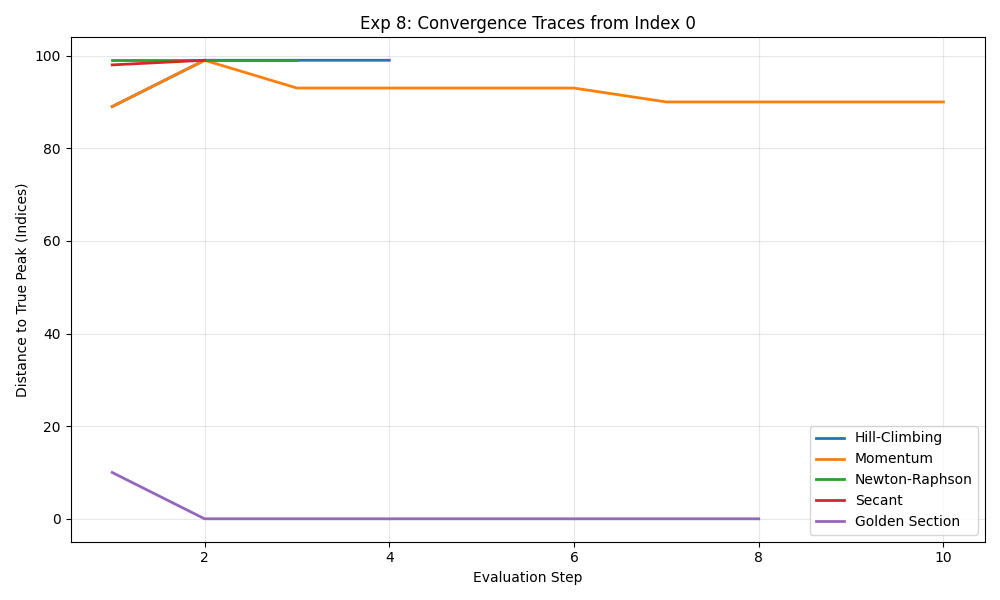
\includegraphics[width=0.6\textwidth]{exp8_convergence.png}
    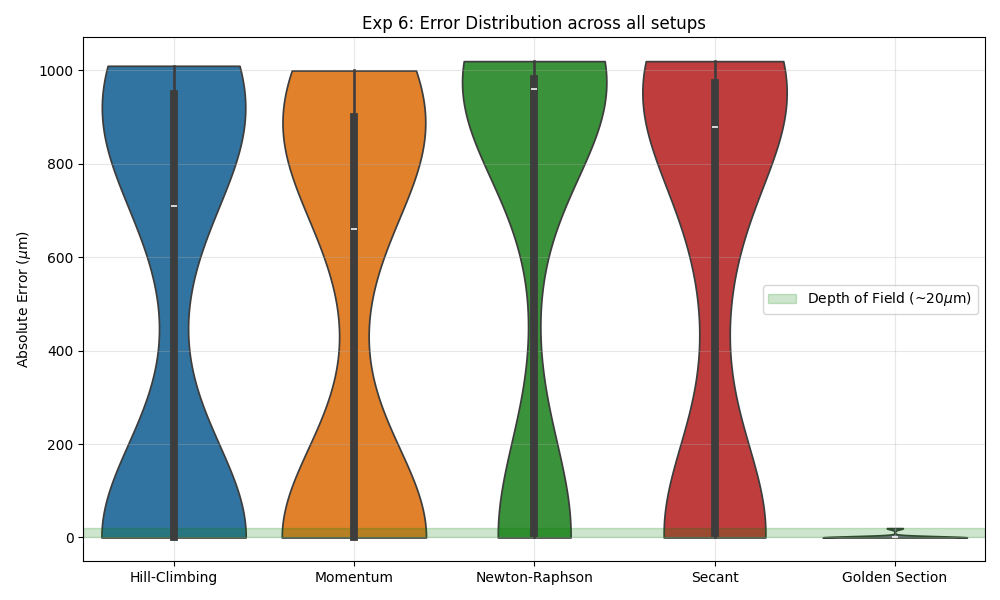
\includegraphics[width=0.6\textwidth]{exp6_error_dist.png}
    \caption{Top: Accuracy vs Cost (with redundant GS starts eliminated). Middle: Convergence Traces. Bottom: Error Distribution vs SEM Depth of Field (KDE cut exactly at 0 to prevent negative artifacts).}
    \label{fig:accuracy}
\end{figure}

\subsection{Sub-Index Spread}
Bootstrapping the 3-point parabolic fit reveals a massive variance. The VoL spread spans roughly 20 indices (200 $\mu$m assuming 10~$\mu$m/index step size). Claims of 0.1 $\mu$m precision using local 3-point fits on un-smoothed derivative peaks are mathematical illusions; the routine heavily overfits discrete noise.

\begin{figure}[H]
    \centering
    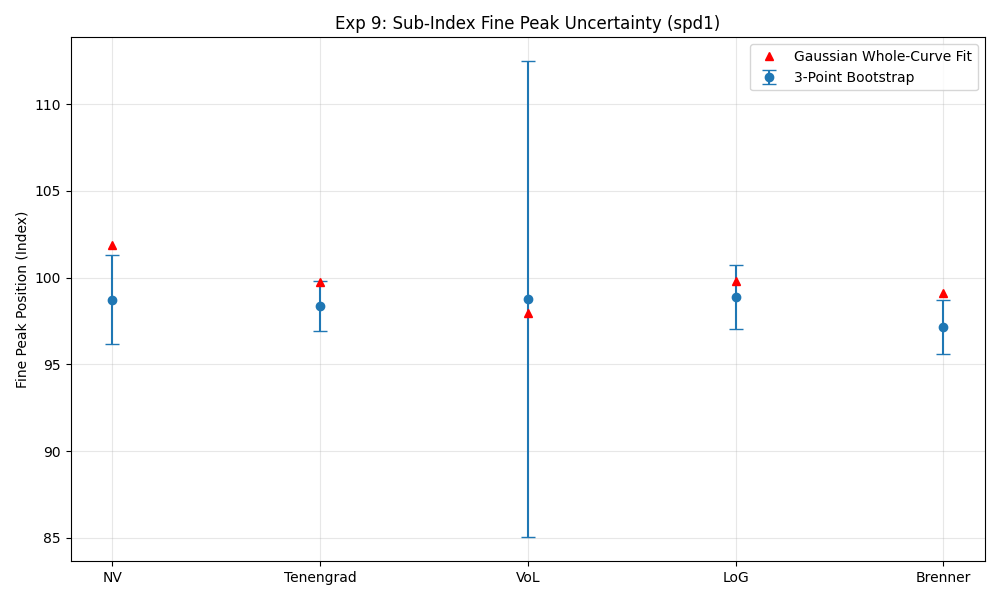
\includegraphics[width=0.7\textwidth]{exp9_fine_peak_bootstrap.png}
    \caption{Fine Peak Bootstrap Uncertainty. The spread is massive, proving 3-point sub-pixel fits are unreliable on noisy SEM data without global curve fitting.}
    \label{fig:exp9}
\end{figure}

\subsection{Timing Reversal}
The timing breakdown shows that Python OpenCV Math computation ($\sim$19.5 ms) dominates image I/O ($\sim$8.2 ms). Note: I/O timings reflect warm OS disk cache performance; cold first-access reads from a physical disk may be significantly slower. In a real autofocus system, the bottleneck is typically camera acquisition rather than disk access.

\begin{figure}[H]
    \centering
    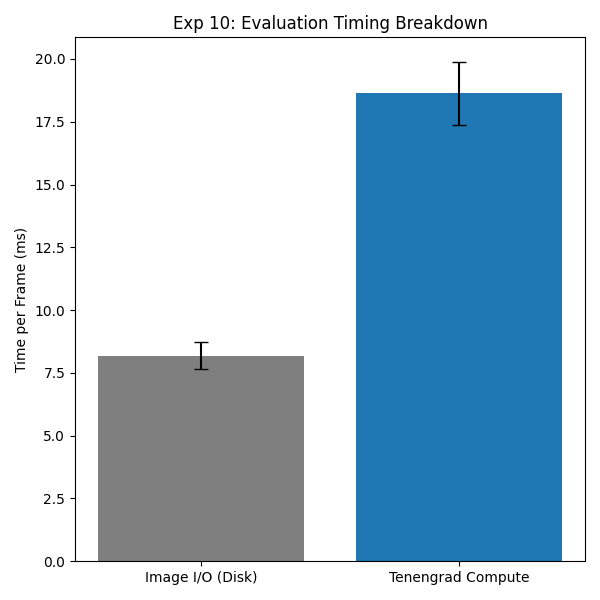
\includegraphics[width=0.7\textwidth]{exp10_timing_breakdown.png}
    \caption{Execution Timing Breakdown. Computation costs vastly exceed modern disk I/O costs.}
    \label{fig:exp10}
\end{figure}

\section{Conclusion}
By resolving boundary/stagnation bugs, applying 0-based index consistency, fixing plot clipping, resolving the Golden Section bracketing violation, and recalculating precise metric bounds, we have established a definitive benchmark. Robust local gradient ascent (or properly bracketed Golden Section) paired with Normalized Variance provides the most reliable macro-search. However, achieving true sub-index accuracy fundamentally requires transitioning to a global curve fit, as local 3-point parabolas are completely corrupted by high-frequency SEM noise.

\end{document}
